%no borrar PREAMBULO
\documentclass[12pt]{article}

\usepackage[top=3.5 cm, bottom=2.5  cm, left=3 cm, right=3 cm]{geometry}
\usepackage{fancyhdr}
\pagestyle{fancy}

\usepackage[hidelinks]{hyperref} %esta opción saca las cajas de colores de los hiperlinks

\fancyfoot[C]{\thepage }  %numera las páginas

\usepackage[utf8]{inputenc}

\usepackage{amsmath,amsfonts,amssymb}
\usepackage{xcolor}
\usepackage{fancyvrb}
\newcommand\verbbf[1]{\textcolor[rgb]{0,0,1}}%comando para colorear el texto en verbatim

%\linespread{1} %por si queremos achicar el espacio entre lineas

\usepackage{tabularx,booktabs}
\usepackage{graphicx}
\usepackage{float} %para que las figuras puedan ponerse en cualquier lado

\usepackage{subcaption}
\usepackage{layout}
\usepackage{multicol}  %para escribir en columnnas 
\usepackage{float}
\usepackage{textcomp}
\usepackage{natbib}
\usepackage{tikz}
\usepackage{multirow} %para cambiar el alto de una fila en una tabla
\tikzset{
  connect/.style = { dashed, gray }
}
\usepackage{pgfplots}
\pgfplotsset{compat=1.8}
\usepackage[english ,spanish]{babel}
\usepackage{latexsym}
\usepackage{verbatim}

%\usepackage{alltt}
\usepackage{indentfirst}

\usepackage{fancybox, calc} 

\usepackage[flushmargin]{footmisc} %para alinear las notas de página

\usepackage{url}
\usepackage{advdate}
\usepackage{wrapfig}
\usepackage{amsthm}
\usepackage[inline]{enumitem} %para hacer listas en una linea, los mismos comandos con *
\newtheorem*{myteo}{Teorema} % la * es para no numerarlos
\newtheorem*{myexample}{Ejemplo}
\newtheorem*{myprop}{Proposición}
\newtheorem*{mylem}{Lema}
\theoremstyle{definition}
\newtheorem*{mydef}{Definición}
\newtheorem{ejer}{Ejercicio}
\newtheorem*{mydefs}{Definiciones}
%\theoremstyle{remark}
\newtheorem*{myobs}{Observación}
\newtheorem*{remark}{Importante}

\renewcommand{\baselinestretch}{1}  %interlineado

\addto\captionsspanish{%
  \renewcommand{\figurename}{Figura}%
}

\newcommand\myText[1]{\text{\scriptsize\tabular[t]{@{}l@{}}#1\endtabular}}
\addto\captionsspanish{%
  \renewcommand{\tablename}{Tabla}%
}

\def \ds {\displaystyle} %define un comando abreviado  
\def\com{“R”}

\usepackage{hyperref}%para referencias de internet con link!
\newcommand*{\fullref}[1]{\hyperref[{#1}]{ \nameref*{#1}}}
%comando \fullref para que ademas del número de capitulo, sección etc. escriba el título del capitulo, sección o lo que sea a lo que estamos haciendo referencia

\newcommand\comentario[1]{\textcolor{red}{#1}}%comentarios en el pdf

\interfootnotelinepenalty=10000 %previene que se pasen a otra página las notas de pie
\raggedbottom 
\addtolength{\topskip}{0pt plus 10pt}
\addtolength{\footnotesep}{0.1mm}

\VerbatimFootnotes%para poder usar Verbatim en las notas de pie

\begin{document}

\fancyhf{}
\pagestyle{fancy}
\lhead{Departamento de Matem\'{a}tica\\Universidad Nacional del Comahue}
\rhead{Matem\'{a}tica 1\\ Licenciatura en Ciencias Biol\'{o}gicas}

%HASTA ACA 

\begin{centering}
\Large{\textbf{Trabajo Práctico N° 4}}\\
%\large{\textbf{Primera Parte}}\\
%\large{\textbf{Números Reales}}\\
\end{centering}
%\vspace{1cm}

\section{Extremos, cotas, conjuntos acotados, Intervalos}

\fbox{ \parbox{0.98\linewidth}{
\noindent
\begin{mydef}  \textbf{Máximo y mínimo, cotas, supremo e ínfimo de un conjunto}\\
\noindent
Sea $A$ un conjunto de números cualesquiera. 
\begin{itemize}
\setlength\itemsep{0em}
\item Diremos que  $M \in A$ es el  \textbf{máximo} del conjunto $A$ si para todo elemento $x \in A$  se verifica que $x \leq M$.
\item Diremos que $m \in A$ es el  \textbf{mínimo} del conjunto $A$ si para todo elemento $x \in A$  se verifica que $x \geq m$.
\item Diremos que $c \in \mathbb{R}$ es una \textbf{cota inferior} del conjunto  $A$ si para todo elemento $x \in A$  se verifica que $x \geq c$.
\item Diremos que $C \in \mathbb{R}$ es una \textbf{cota superior} del conjunto  $A$ si para todo elemento $x \in A$  se verifica que $x \leq C$.
\item Llamaremos \textbf{ínfimo} del conjunto $A$ a su máxima cota inferior.
\item Llamaremos \textbf{supremo} del conjunto $A$ a su mínima cota superior .
\item Un conjunto que tiene cotas superiores se dice \textbf{acotado superiormente}.
\item Un conjunto que tiene cotas  inferiores se dice \textbf{acotado inferiormente}.
\item Un conjunto $A$ se dice \textbf{acotado} si lo es superior e inferiormente.
\end{itemize}
\end{mydef}
}}


\begin{enumerate}
%1
\item Para los siguientes conjuntos determinar, de ser posible:
\begin{multicols}{3}
\begin{itemize}
\setlength\itemsep{0em}
\item Dos cotas superiores.	
\item Dos cotas inferiores.		
\item El supremo.	
\item El ínfimo.
\item El máximo.
\item El mínimo.
\end{itemize}
\end{multicols}
\begin{multicols}{2}
\begin{enumerate}
\setlength\itemsep{0em}
\item $\{-3, -2, 1, 2\}$
\item $\{x \in \mathbb{R} / x-2 < 1\}$
\item $[-2,4)$
\item $\{x \in \mathbb{R} / -x^2+ 3x > 0\}$
\item $(-\infty, 4]$
\item $(-\infty, 4)$
\item $\{x \in \mathbb{R} / -x^2+ 3x > 1\}$
\item $\mathbb{N}$ 
\item $\mathbb{Z}$
\item $[-3,2] \cup [4, 6]$
\item $[2, +\infty)$
\item $\{x \in \mathbb{R} / -x^2+ 3x < 0\}$
\end{enumerate}
\end{multicols}
En caso de no ser posible, explicar por qué.
\vspace{1cm}

%2
\item Analizar si las siguientes proposiciones son verdaderas o falsas, y justificar:
\begin{enumerate}
\setlength\itemsep{0em}
\item Todo conjunto finito tiene siempre máximo y mínimo.
\item Todo conjunto finito es acotado. 
\item Todo conjunto acotado es finito.
\item Si un conjunto es infinito, no es acotado. 
\item Si un conjunto posee máximo, es acotado superiormente.
\item Si un conjunto es acotado superiormente, posee máximo.
\item Todo intervalo cerrado es acotado.
\item Todo intervalo cerrado posee siempre máximo y mínimo.
\item Todo conjunto acotado posee supremo e ínfimo.
\item Todo conjunto acotado posee máximo y mínimo.
\item El supremo de un conjunto acotado pertenece siempre al conjunto.
\end{enumerate}

%3
\item Proponer ejemplos de conjuntos en los cuales ninguna de las cotas superiores o inferiores pertenezcan al conjunto y ejemplos de conjuntos en los cuales haya al menos una cota superior o inferior perteneciente al conjunto.

%4
\item Considerar la proposición \textbf{p}: un conjunto A se dice acotado si lo es superior e inferiormente.  
\begin{enumerate}
\setlength\itemsep{0em}
\item Escribir la negación: $\sim \mathbf{p}$.
\item Dar ejemplos de conjuntos no acotados.
\end{enumerate}

\fbox{ \parbox{0.98\linewidth}{ %para hacer el recuadro del ancho de página
%Definicion
\noindent
\begin{mydef} \textbf{Intervalos acotados.}\\
\noindent
Sean dos números reales $a$ y $b$ tales que $a < b$.
\begin{itemize}
\setlength\itemsep{0em}
\item Se llama \textbf{intervalo abierto} $(a,b)$ al conjunto de números reales comprendidos entre $a$ y $b$, sin incluir a estos últimos. En  símbolos:
\begin{equation*}
(a,b) = \{x \in \mathbb{R}/ a < x < b\}
\end{equation*}
\item Análogamente, se llama \textbf{intervalo cerrado} $[a,b]$ al conjunto de números reales comprendidos entre $a$ y $b$, incluyendo a estos últimos. En  símbolos:
\begin{equation*}
[a,b] = \{x \in \mathbb{R}/ a \leq x \leq b\}
\end{equation*}
\item Análogamente pueden definirse también los intervalos semicerrados o semiabiertos, los cuales son abiertos a izquierda y cerrados a derecha o viceversa.
\end{itemize}
\end{mydef}
}}  %termina el recuadro
%5
\item Escribir las definiciones anteriores (intervalos abiertos y cerrados) como conjunción o disyunción de proposiciones.

%6
\item  Escribir en símbolos las definiciones de intervalos semiabiertos.  Escribirlas también como conjunción o disyunción de proposiciones.

\fbox{ \parbox{0.98\linewidth}{
%Definicion
\noindent
\begin{mydef} \textbf{Intervalos no acotados.}\\
\noindent
Se llaman intervalos no acotados a los siguientes conjuntos de números reales:
\begin{multicols}{2}
\begin{itemize}
\setlength\itemsep{0em}
\item $(- \infty,a) = \{x \in \mathbb{R}/  x < a\}$	
\item $(- \infty,a] = \{x \in \mathbb{R}/  x \leq a\}$	
\item $(a, +\infty) = \{x \in \mathbb{R}/  x > a\}$	
\item $[a, +\infty) = \{x \in \mathbb{R}/  x \geq a\}$	
\item $(-\infty, \infty) = \mathbb{R}$	
\end{itemize}
\end{multicols}
\end{mydef}
}}

%7 se juntó con el ex 9

%7
\item  Decir si los siguientes conjuntos son intervalos o no lo son y justificar:
\begin{multicols}{2}
\begin{enumerate}
\setlength\itemsep{0em}
\item $A = \{x \in \mathbb{R} / x \leq 2\}$
\item $A = \{x \in \mathbb{R} / x \leq 2 \wedge x \geq 0\}$
\item $A = \{x \in \mathbb{R} /  x \leq 2 \wedge x \geq 6\}$
\item $A = \{x \in \mathbb{R} /  x \leq 2 \vee x \geq 6\}$
\end{enumerate}
\end{multicols}

\fbox{ \parbox{0.98\linewidth}{ %para hacer el recuadro del ancho de página
%Remark
\noindent
\begin{remark}
\noindent
No cualquier conjunto de números reales es un intervalo. Sólo son intervalos los siguientes conjuntos:
\begin{multicols}{5}
\begin{itemize}
\setlength\itemsep{0em}
\item $[a,b]$  
\item $(a,b)$
\item $[a,b)$ 
\item $(a,b]$
\item $(-\infty ,a)$
\item $(-\infty ,a]$ 
\item $(a,+\infty )$ 
\item $[a,+\infty )$
\item $ \mathbb{R}$
\item $\varnothing$
\end{itemize}
\end{multicols}

Cualquier conjunto que no sea uno de los anteriores no es un intervalo.
\end{remark}
}}
%8
\item  Representar gráficamente los siguientes conjuntos y escribirlos con notación conjuntista: 
\begin{multicols}{3}
\begin{enumerate}
\setlength\itemsep{0em}
\item $(-2,3)$ 
\item $[4,9)$
\item $[-3,9]$
\item $[-1,3]$	
\item $(-\infty,2]$	
\item $(-1, +\infty)$	
\item $(-\infty,4)$
\item $[-2,+\infty)$ 
\end{enumerate}
\end{multicols}

%9 Nuevo
\item  Para los intervalos del ejercicio anterior, decir si se trata de intervalos acotados o no. Dar, si corresponde, cotas superiores, inferiores, máximo, mínimo, supremo e ínfimo.

%10
\item  Proponer un ejemplo de un conjunto tal que (uno para cada ítem):
\begin{enumerate}
\setlength\itemsep{0em}
\item tenga máximo pero no mínimo.
\item tenga cotas superiores pero no máximo. 
\item sea acotado inferiormente pero no sea un intervalo.
\end{enumerate}


%Definicion
\fbox{ \parbox{0.98\linewidth}{
\noindent
\begin{mydef} \textbf{Operaciones con intervalos.\\}
\noindent
Sean A y B dos intervalos cualesquiera dentro de un referencial R. Definiremos las siguientes operaciones:
\begin{itemize}
\setlength\itemsep{0em}
\item La \textbf{unión} de $A$ y $B$ es el conjunto formado por todos los elementos comunes y no comunes que pertenecen a $A$ y a $B$. En símbolos:
\begin{equation*}
	A \cup B = \{ x \in A \vee x \in B\}
\end{equation*}
\item La \textbf{intersección} de $A$ y $B$ es el conjunto formado por los elementos comunes a $A$ y a $B$. En símbolos:
\begin{equation*}
	A \cap B = \{ x \in A \wedge x \in B\}
\end{equation*}
\item La \textbf{diferencia} entre $A$ y $B$ es el conjunto formado por los elementos que pertenecen a $A$ y no pertenecen a $B$. En símbolos:
\begin{equation*}
	A - B = \{ x \in A \wedge x \not \in B\}
\end{equation*}
\item El \textbf{complemento} de $A$ es el conjunto formado por los elementos del referencial que no pertenecen a $A$. En símbolos:
\begin{equation*}
	\bar{A} = \{ x \in R / x \not \in A\}
\end{equation*}
\end{itemize}
\end{mydef}
}}  %termina el recuadro

%11
\item Representar gráficamente y calcular $A \cup B$, $A\cap B$, $A-B$ y $B-A$ siendo:
\begin{multicols}{2}
\begin{enumerate}
\setlength\itemsep{0em}
\item $A = (-2, 4)$ y $B = (1,5)$
\item $A = (-2, 0]$ y $B = (1,5)$
\item $A = [-2, 8]$ y $B = (1,5)$
\item $A = (-1, 4]$ y $B = (4,5)$
\item $A = (-1, 4]$ y $B = [4,5)$
\item $A = (4, +\infty)$ y $B = (-\infty,5)$
\item $A = (-\infty, 0)$ y $B = [-1,1]$
\item $A = (-\infty, 0]$ y $B = [0,+\infty)$
\end{enumerate}
\end{multicols}

%12
\item Para cada uno de los conjuntos obtenidos como resultado de las operaciones del ejercicio anterior, decir si son acotados o no. Si tienen, indicar dos cotas superiores, dos cotas inferiores, supremo, ínfimo, máximo y mínimo.

\noindent
\section{Funciones acotadas, extremos de una función}
\fbox{ \parbox{0.98\linewidth}{ %para hacer el recuadro del ancho de página
%Definicion
\noindent
\begin{mydef} \textbf{Funciones acotadas.}\\
\noindent
Una función se dice \textbf{acotada} si lo es su conjunto imagen. Según sean las características del conjunto imagen se pueden definir también funciones \textbf{acotadas inferiormente} y \textbf{acotadas superiormente}.
\end{mydef}
}}  %termina el recuadro

%13
\item Dar ejemplos gráficos de funciones tales que: 
\begin{enumerate}
\setlength\itemsep{0em}
\item Sean acotadas (superior e inferiormente),
\item Sólo sean acotadas inferiormente,
\item Sólo sean acotadas superiormente,
\item No tengan cotas ni superiores ni inferiores.
\end{enumerate}
Cuando corresponda indicar algunas cotas.\\
%\vspace{0.5cm}
\fbox{ \parbox{0.98\linewidth}{ %para hacer el recuadro del ancho de página
%Definicion
\noindent
\begin{mydef} \textbf{Extremos de una función.}
\noindent
\begin{itemize}
\setlength\itemsep{0em}
\item Se dice que una función $f$ alcanza en un punto $x_{0}$ de su dominio un \textbf{máximo absoluto} $M$,  si $M = f(x_{0})$ es mayor o igual que la imagen de cualquier otro elemento del dominio. En símbolos:\\
$M = f(x_{0})$ es un máximo absoluto de $f$ si para todo $x \in Dom(f)$ se verifica $f(x)\leq M$.

El número real $M$  es el máximo del conjunto de las imágenes.
\item Se dice que una función $f$ alcanza en un punto $x_{0}$ de su dominio un \textbf{mínimo absoluto} $m$,  si $m = f(x_{0})$ es menor o igual que la imagen de cualquier otro elemento del dominio. En símbolos:\\
$m = f(x_{0})$ es un mínimo absoluto de $f$ si para todo $x \in Dom(f)$ se verifica $f(x)\geq m$.

El número real  $m$  es el mínimo del conjunto de las imágenes.
\end{itemize}
\end{mydef}
}}  %termina el recuadro


%14
\item Analizar si las siguientes proposiciones son verdaderas o falsas, y justificar:
 \begin{enumerate}
\setlength\itemsep{0em}
\item Si una función es acotada (superior e inferiormente), necesariamente tiene máximo y mínimo absolutos.
\item Si una función tiene máximo y mínimo absolutos, necesariamente es acotada.
\item Ninguna función polinómica es acotada. 
\item La función $f(x) = sen(x)$ es acotada.
\item La función $f(x) = tg(x)$ es acotada.
\item Las funciones exponenciales $f(x) = a.e^x$ son acotadas sólo superior o inferiormente.
\item Las funciones logarítmicas $f(x) = a. ln(x)$ son acotadas sólo superior o inferiormente.
\end{enumerate}
\item  Para cada uno de los siguientes incisos, se pide:
\begin{itemize}
\item Graficar ambas funciones (podés usar un graficador).
\item Encontrar analíticamente los puntos de intersección (capaz no dan números muy redonditos). Acá toca hacer cuentas.
\item  Indicar en el gráfico los intervalos del dominio donde $f(x) < g(x)$. Escribir esto usando intervalos (o unión de ellos).
\item  Indicar en el gráfico los intervalos del dominio donde $f(x) > g(x)$. Escribir esto usando intervalos(o unión de ellos).
\item  Indicar en los dos incisos anteriores cuál sería la solución si las desigualdades fueran $\leq$ o $\geq$.
\end{itemize}
\begin{enumerate}
\item $f(x) = x^2 - 2x$ y $g(x) = x - 2$
\item $f(x) = x^2 - 2x - 3$ y $g(x) = -x - 3$
\item $f(x) = x^2 - 4$ y $g(x) = 2x - 1$
\item $f(x) = 2x^2 + 6x$ y $g(x) = 2x$
\item $f(x) = x^2 + 5x + 4$ y $g(x) = -\frac{5}{2}x - 5$
\end{enumerate}

\noindent
\section{Desigualdades. Comparación entre funciones}
%15
\item  Para cada uno de los siguientes incisos, llevar a una comparación con cero si no está así, factorizar lo que haga falta y lo que se pueda, y buscar el resultado analizando el signo de cada factor. Escribir los conjuntos solución utilizando intervalos (o unión de ellos):
\begin{enumerate}
\begin{multicols}{2}
\item $2 + 3x < 5$
\item $ -2x^2 + 4x \geq 0$
\item $ x^2 - 4 \leq 0$
\item $ \frac{x^2 - 4 }{x(x - 4)} > 0$
\item $x^3 - 9x^2 > 0$
\item $(2-x)(3x+2) < 0$
\item $5x - 2x^2 \leq 3$
\item $12x^2+6x < x +2$
\end{multicols}

\end{enumerate}
%16
\item  Hallar el dominio de validez de cada una de las siguientes desigualdades. Si es posible, expresarlo como intervalo o unión de intervalos. Usar el método que más te guste (graficando las funciones a comparar o analizando signos de factores):
\begin{enumerate}
\begin{multicols}{2}
\setlength\itemsep{0em}
\item $3x - (8-x) > -2$
\item$2x+1 > x-3$
\item $x^2+1 > 4x$
\item $x + \frac{1}{x} \geq 1$
\item $5x(x-3)^2 < 0$
\item $x^2 - 1 \leq 0$
\item $ \frac{x}{x+5} > 0$
\item $ \frac{1}{x-1} >2$
\item $ \frac{x^2-4x}{x+2} \geq 0$
\item $(x-1)(x+2)(x-3) \geq 0$
\item $ \frac{x(x+2)}{x-2} \leq 0$
\item $ \frac{2}{x-2} \geq \frac{3}{x+2}$
\item $ \frac{2}{x-1} - \frac{x}{x+1} \leq 1$
\item $ x^2-4x \leq -1-2x$
\end{multicols}
\end{enumerate}
%17
\item Para resolver la desigualdad $\frac{3}{x} < 2$ una persona procede así:\\
Multiplica por $x$ de ambos lados de la desigualdad, y obtiene: $ 3 < 2x$. Luego divide todo por $2$ y resulta $ \frac{3}{2} < x$ de donde deduce que el dominio de validez de la desigualdad es el intervalo $(\frac{3}{2},+\infty)$.  \\
El razonamiento es incorrecto. ¿Por qué?. Hacerlo bien.

%18
\item Una de las aplicaciones más directas de las desigualdades es en la determinación del dominio de funciones. Entonces, encontrar el dominio de definición de cada una de las siguientes funciones, y escribirlo como intervalo o unión de intervalos.
\begin{enumerate}
\begin{multicols}{2}
%\setlength\itemsep{0em}
\item $f(x) = \sqrt{1-x}$
\item$f(x) = \sqrt{2x+3}$
\item$f(x) = \sqrt{x(x+3)}$
\item $ f(x) = \frac{x-2}{x^3-x^2}$
\item $ f(x) = \sqrt{\frac{x-2}{x^3-x^2}}$
\item$f(x) = \log{(2x+3).(x-1)}$

\end{multicols}
\end{enumerate}

\section{Valor absoluto. El valor absoluto como distancia}

\fbox{ \parbox{0.98\linewidth}{ %para hacer el recuadro del ancho de página
%Definicion 
\noindent
\begin{mydef} \textbf{Valor absoluto de un número real.\\}
\noindent
Se define el \textbf{valor absoluto} de un número real $x \in \mathbb{R}$ de la siguiente manera:
\begin{equation*}
     | x | = \left \{
	\begin{aligned}
	x  \text{ si }  x \geq 0\\
	-x \text{ si } x < 0
	\end{aligned}
	\right.
\end{equation*}
\end{mydef}
}}  %termina el recuadro


%19
\item Dar la interpretación geométrica del valor absoluto de un número real, interpretándolo en términos de distancia.

%20
\item Hallar si es posible el o los valores de x que satisfacen las siguientes expresiones y graficar la solución en la recta real: 
\begin{multicols}{4}
\begin{enumerate}
\setlength\itemsep{0em}
\item $|x| = 3$
\item $|x| = 0$
\item $|x| > 0$
\item $|x| < 1$
\end{enumerate}
\end{multicols}

%17
\item  Interpretar las siguientes expresiones en términos de distancia, graficar y dar el conjunto solución (cuando corresponda) como intervalos o unión de  intervalos:
\begin{multicols}{4}
\begin{enumerate}
\setlength\itemsep{0em}
\item $|x-2| = 1$
\item $|x+1| = 3$
\item $|x-c| = 2$
\item $|x-3| = d$
\item $|x-2| < 1$
\item $|x+1| < 3$
\item $|x-c| < 2$
\item $|x-3| < d$
\item $|x-2| > 1$
\item $|x+1| > 3$
\item $|x-c| > 2$
\item $|x-3| > d$
\item $|x-3| \geq 1$
\item $|x+3| \leq 2$
\item $|x| < 2$
\item $|x| \geq 3$
\end{enumerate}
\end{multicols}


%18
\item Considerar los siguientes conjuntos. Primero graficar y pensarlos en términos de distancia. Luego escribir simbólicamente esa distancia usando el módulo.
\begin{enumerate}
\setlength\itemsep{0em}
\item Puntos de la recta que distan de $2$ exactamente $5$ unidades.
\item Puntos de la recta que distan de $3$ en menos de $2$ unidades.
\item Puntos de la recta que distan de $1$ en $3$ unidades o más.
\item Puntos de la recta que distan de $-2$ exactamente $3$  unidades.
\item Puntos de la recta que distan de $-4$ menos de $2$ unidades.
\item Puntos de la recta que distan de $-5$ en más de $3$ unidades.
\item Puntos de la recta que distan de $0$ exactamente $5$ unidades.
\item Puntos de la recta que distan de $0$ en $3$ unidades o menos.
\item Puntos de la recta que distan de $0$ en más de $4$ unidades.
\item Puntos de la recta que distan de $2$ en  menos de  $5$ y más de $3$ unidades.
\item $\{ x \in \mathbb{R}$ tales que $x \in (c -1, c+1)\}$
\item $\{ x \in \mathbb{R}$ tales que $x \in (-\infty, -2) \cup (2, + \infty)\}$
\item $\{ x \in \mathbb{R}$ tales  que $x \neq 0\}$
\item $\{ x \in \mathbb{R}$ tales  que $x \neq 3\}$
\item $\{ x \in \mathbb{R}$ tales  que $x \in (-4, -2) \cup (2, 4)\}$
\item $\{ x \in \mathbb{R}$ tales  que $x \in [c - 1, c+1]\}$
\item $\{ x \in \mathbb{R}$ tales  que $x \in (- \infty, -2] \cup [2, +\infty)\}$
\item $\{ x \in \mathbb{R}$ tales  que $x \in [- 4, -2) \cup (2, 4]\}$
\end{enumerate}

\section{Función valor absoluto}

\fbox{ \parbox{0.98\linewidth}{
\noindent
\begin{mydef}  \textbf{Función Valor Absoluto (o Función Módulo)}\\
\noindent
La función \textbf{valor absoluto} se define de la siguiente manera:
\begin{equation*}
         f:   \mathbb{R}  \rightarrow \mathbb{R}^{+} \cup \{  0 \}
\end{equation*}
\begin{equation*}
        x  \rightarrow | x |
\end{equation*}
\begin{equation*}
         f(x) = | x | = \left \{
	\begin{aligned}
	x  \text{ si }  x \geq 0\\
	-x \text{ si } x < 0
	\end{aligned}
	\right.
\end{equation*}
\end{mydef}
}}

%1
\item Representar gráficamente  $f(x) = |x|$
%2
\item El siguiente es el gráfico de $f(x)$
\begin{figure}[H]
\centering
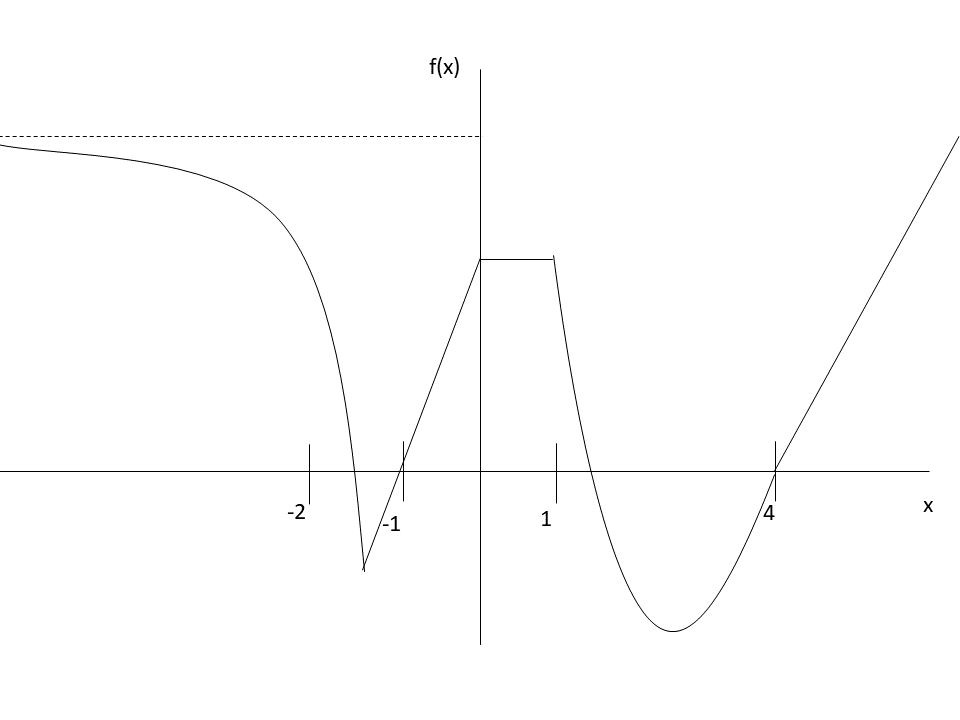
\includegraphics[width=0.5\textwidth]{TP2-1.png}
\end{figure}

\begin{enumerate}
\item Dibujar el gráfico que corresponde a $|f(x)|$ 
\item Indicar el o los intervalos donde $|f(x)| = f(x)$ 
\item Indicar los intervalos donde $|f(x)| = -f(x)$ 
\end{enumerate}

\item Para cada una de las siguientes funciones se pide:
\begin{enumerate}
\item Graficar $f(x)$ 
\item Graficar $|f(x)|$ y llamarla $g(x)$ 
\item En la función módulo, indicar sobre el gráfico, cuál es el valor de la función en cada intervalo del dominio definido por el módulo. Nombrar esos intervalos.
\item Desdoblar el módulo de acuerdo a la definición y comparar con lo analizado en el inciso anterior
\end{enumerate}
\noindent
%\fbox{ \parbox{0.98\linewidth}{
Por ejemplo: para $f(x) = x+2$, $g(x) = |x + 2|$ \\
\begin{equation*}
        g(x) = x + 2  \text{ en }  [ -2,+\infty)   \text{ y }  g(x) = -(x + 2)  \text{ en }  (-\infty, -2) 
\end{equation*}
\vspace{0.3 cm}
\begin{multicols}{2}
\begin{figure}[H]
\centering
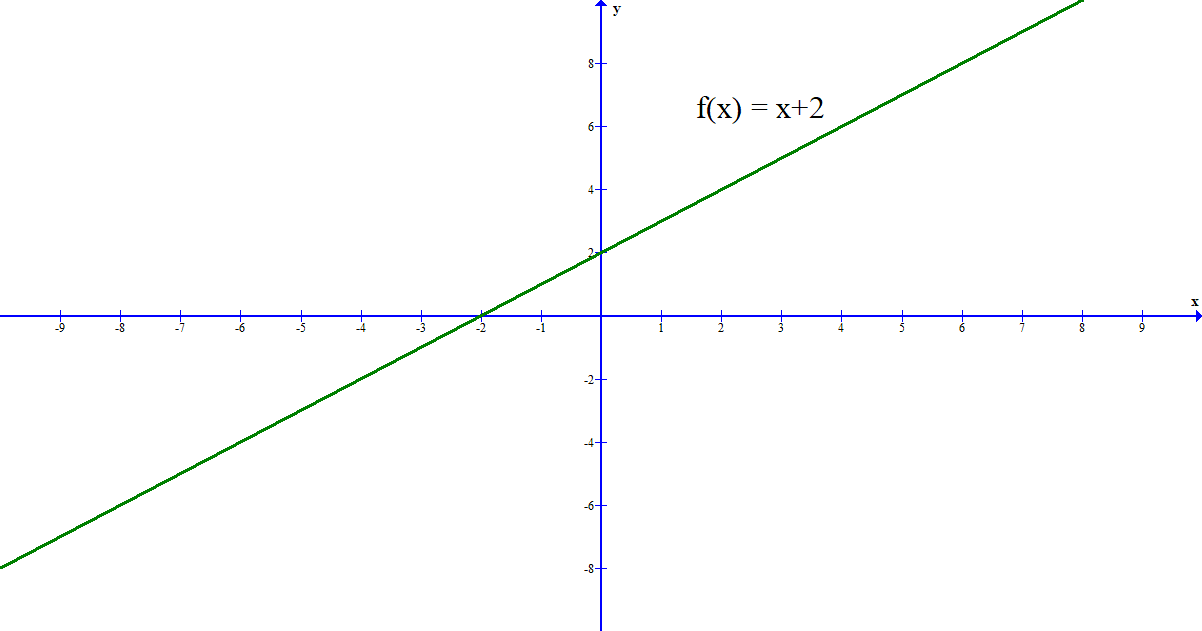
\includegraphics[width=0.5\textwidth]{X+2.png}
\end{figure}
\begin{figure}[H]
\centering
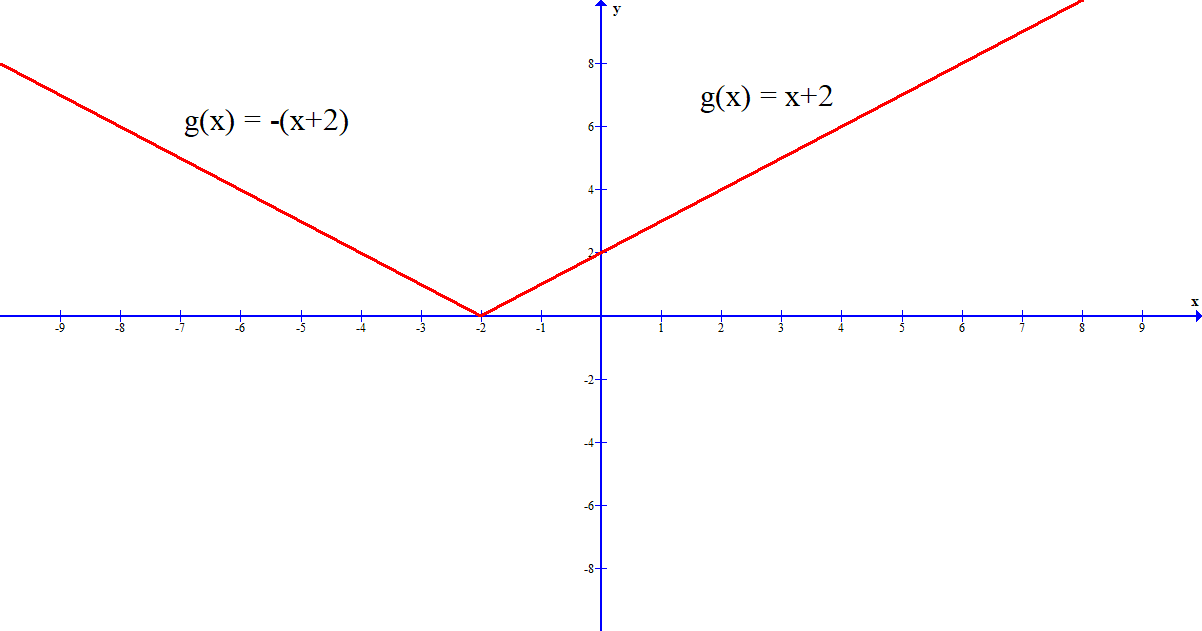
\includegraphics[width=0.5\textwidth]{MODX+2.png}
\end{figure}
\end{multicols}
\noindent
De acuerdo a la definición de la función módulo:
\begin{equation*}
         g(x) = |x +2| = \left \{
	\begin{aligned}
	x+2  \text{ si }  x \in [ -2,+\infty) \\
	-(x+2) \text{ si } x \in (-\infty, -2)
	\end{aligned}
	\right.
\end{equation*}
%}
\begin{multicols}{2}
\begin{enumerate}
\item $f(x) = 2x-1$ 
\item $f(x) = x^{2}-2x$ 
\item $f(x) = (x-1).(x-2)$ 
\item $f(x) = x^{3}-1$ 
\item $f(x) = \sin x$ si $x \in [0, 2\pi]$
\item $f(x) =\cos x$ 
\item $f(x) =\frac{1}{x}$ 
\item $f(x) = -4-3x$ 
\item $f(x) =9-x^{2} $ 
\item $f(x) =\frac{1}{2-x}$ 
\item $f(x) = x.(x-1).(x+1)$
\item $f(x) =  \ln x$  
\end{enumerate}
\end{multicols}

\item  Hallar los valores de $x$ que satisfacen las siguientes expresiones, interpretándolas gráficamente como comparación de funciones:
\begin{multicols}{2}
\begin{enumerate}
\item $|x-1|=3$ 
\item $|x-5| <2$ 
\item $0 < |x+3|<2$ 
\item $|2x-4| \geq 3$ 
\end{enumerate}
\end{multicols}


\item  A un alumno (que desaprobó)  se le pidió encontrar los puntos de intersección entre las funciones: $f(x) = | x^{2}-2x|$ y $g(x) = x-1$.  Para ello resolvió las siguientes ecuaciones:
\begin{equation*}
  	x^{2}-2x = x-1   \text{   y    } -(x^{2}-2x) = x-1
\end{equation*}
\noindent
De cada igualdad encontró dos puntos de intersección. (Hacer las cuentas). Sin embargo, cuando realiza la gráfica (hacerla) nota que $f(x)$ y $g(x)$ sólo tienen dos puntos de intersección. ¿Por qué razón el alumno encontró cuatro puntos cuando en realidad son sólo dos? ¿Qué omitió en su razonamiento?

\item  Encontrar los puntos de intersección de las siguientes funciones, tanto gráfica como analíticamente, y en este último caso tener en consideración las restricciones correspondientes a cada ecuación:
\begin{multicols}{2}
\begin{enumerate}
\item $f(x) = |x-1|$ y $g(x) = x^{2}-4$
\item $f(x) = x-1 $ y $ g(x) = |x^{2}-4| $
\item $f(x) = |2x-1|$ y $g(x) = (2-x).x $
\item $f(x) = 2x-1$ y $g(x) = |(2-x).x| $
\end{enumerate}
\end{multicols}

\item Considerar las funciones  $|f(x)| = |x^{2}-4|$ y $g(x) = 2x-1$
\begin{enumerate}
\item realizar un gráfico de ambas funciones (mejor en un mismo gráfico)
\item Para $|f(x)|$ definir la función en cada tramo del gráfico (es decir, a qué es igual $|f(x)|$ según si las imágenes de $f(x)$ son positivas o negativas)
\item Encontrar los puntos de intersección entre $|f(x)|$ y $g(x)$ (analíticamente)
\item Señalar en el eje $x$ de este gráfico, el conjunto de puntos para los cuales es $|f(x)| \geq g(x)$.
\item Escribir lo anterior usando intervalos (o unión de ellos)
\end{enumerate}
 

\item Para las desigualdades que siguen:
\begin{itemize}
\item Graficar las funciones que representan cada lado de la desigualdad
\item Proceder como en el ejercicio anterior para determinar el conjunto solución
\end{itemize}
\begin{multicols}{2}
\begin{enumerate}
\item $|x-2| < 2x-1$
\item $|3-x| > 1 - 2x $
\item $3x-4 <|5x-1| $
\item $6x-2 <|6x| $
\item $ |2x-1|\geq x^{2}+2 $
\item $ 3x-4 > |2x - 2x^{2}$
\item $ |x^{2}-42 |\leq -2x+4 $
\item $ |x^{2}-x-6 |\geq x^{2}-1 $
\item $ 2x-1 \geq |(2-x).x|$
\item $ x^{2}-x <|2x+4|$

\end{enumerate}
\end{multicols}

\end{enumerate}

\end{document}
